\documentclass[english,11pt]{beamer}

\DeclareMathOperator{\Cov}{Cov}
\DeclareMathOperator{\Var}{Var}
\DeclareMathOperator{\E}{\mathbb{E}}
\DeclareMathOperator{\Proba}{\mathbb{P}}

\newcommand{\Covb}[2]{\ensuremath{\Cov\!\left[#1,#2\right]}}
\newcommand{\Eb}[1]{\ensuremath{\E\!\left[#1\right]}}
\newcommand{\Pb}[1]{\ensuremath{\Proba\!\left[#1\right]}}
\newcommand{\Varb}[1]{\ensuremath{\Var\!\left[#1\right]}}

% norm
\newcommand{\norm}[1]{\| #1 \|}

\newcommand{\indep}{\rotatebox[origin=c]{90}{$\models$}}





\usepackage{mathptmx,amsmath,amssymb,graphicx,bibentry,bbm,babel,ragged2e}

\makeatletter

\newcommand{\noun}[1]{\textsc{#1}}
\newcommand{\jitem}[1]{\item \begin{justify} #1 \end{justify} \vfill{}}
\newcommand{\sframe}[2]{\frame{\frametitle{#1} #2}}

\newenvironment{centercolumns}{\begin{columns}[c]}{\end{columns}}
%\newenvironment{jitem}{\begin{justify}\begin{itemize}}{\end{itemize}\end{justify}}

\usetheme{Warsaw}
\setbeamertemplate{footline}[text line]{}
\setbeamercolor{structure}{fg=purple!50!blue, bg=purple!50!blue}

\setbeamersize{text margin left=15pt,text margin right=15pt}

\setbeamercovered{transparent}


\@ifundefined{showcaptionsetup}{}{%
 \PassOptionsToPackage{caption=false}{subfig}}
\usepackage{subfig}

\usepackage[utf8]{inputenc}
\usepackage[T1]{fontenc}

\usepackage{multirow}


\makeatother

\begin{document}





\title{A multi-dimensional percolation approach to characterize sustainable mega-city regions}

\author{J.~Raimbault$^{1,2,\ast}$\\
\texttt{juste.raimbault@polytechnique.edu}
}


\institute{$^{1}$Complex Systems Institute, Paris, UPS CNRS 3611 ISC-PIF\\
$^{2}$UMR CNRS 8504 G{\'e}ographie-cit{\'e}s
}


\date{MARAMI 2018\\\smallskip
Avignon\\\smallskip
October 18th 2018
}

\frame{\maketitle}




\sframe{Networks and territories}{

% Keywords : }\textit{Road network; multilayer percolation; mega-city region}

% - intro : LGV ? Avignon : travaux Claire ! - truc avec les Papes ? 
% https://www.persee.fr/doc/anami_0003-4398_1985_num_97_172_2228_t1_0446_0000_3
% https://www.persee.fr/doc/mefr_0223-5110_1984_num_96_1_2762

% -> visu OSM : see Metropolitan region ; plus positioning of Avignon ; Q of sustainibility ?

\centering

	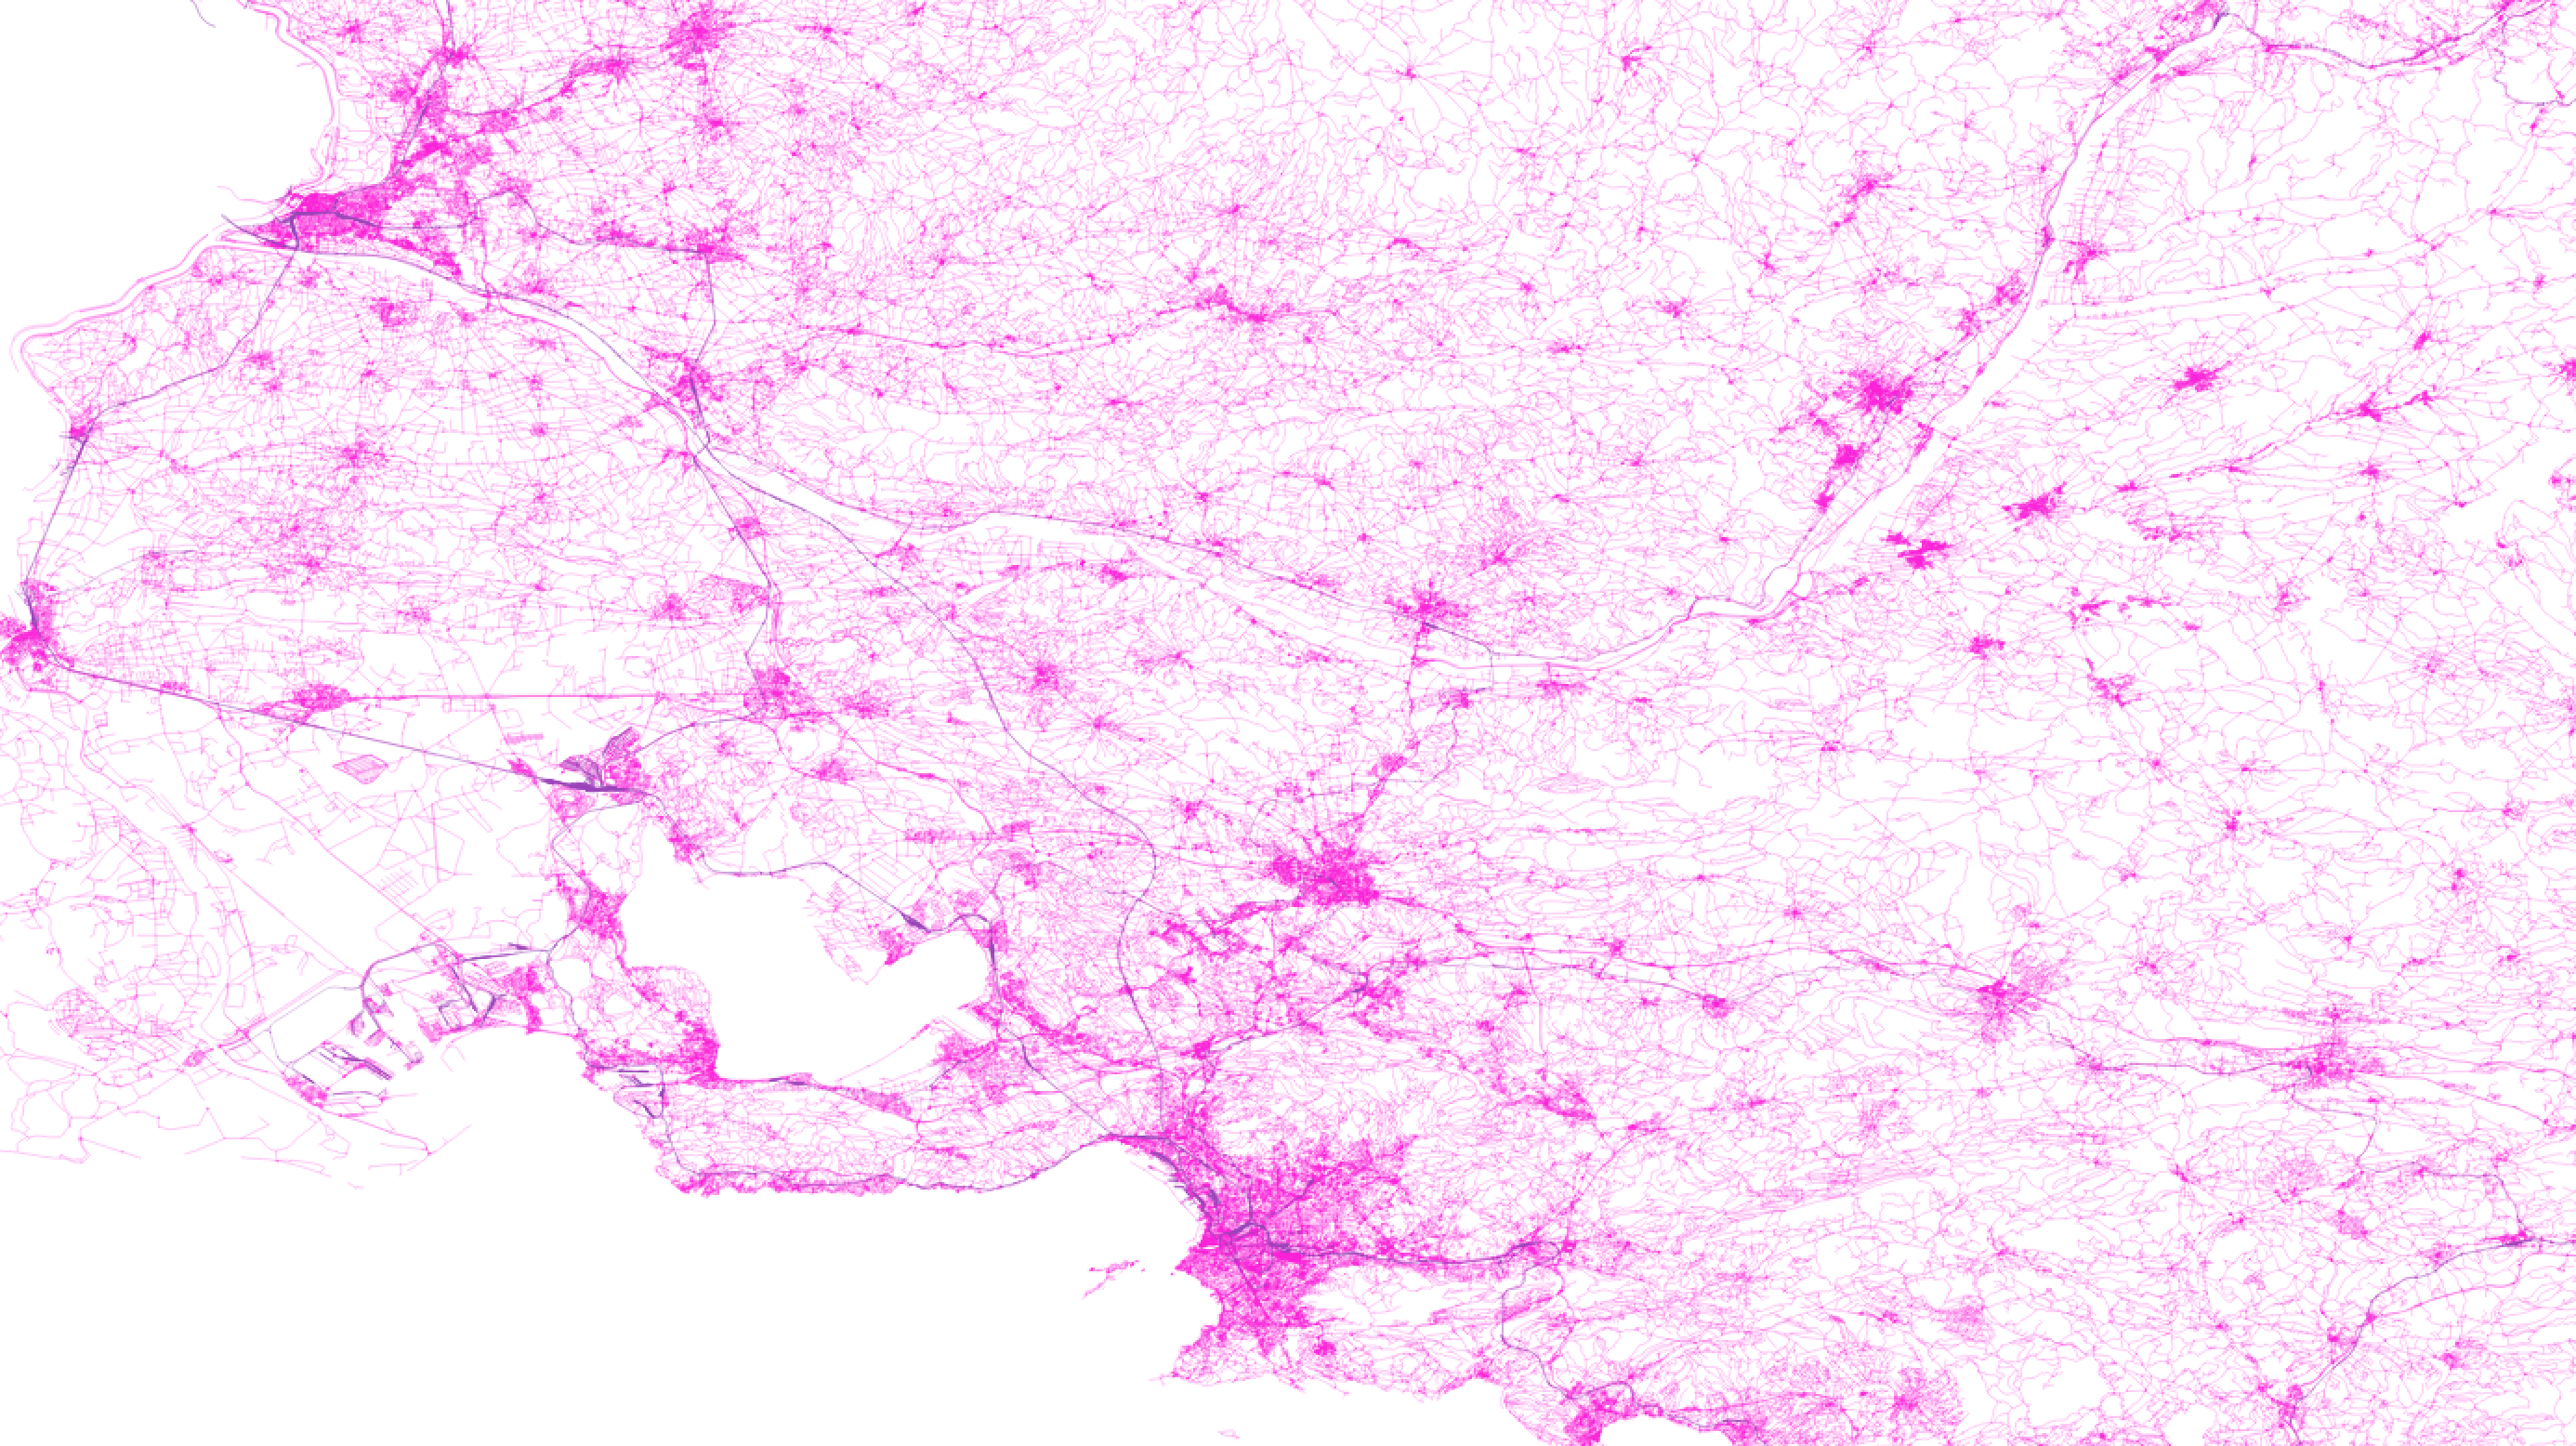
\includegraphics[width=1.2\textwidth]{figures/roadssouth.png}
	
	\footnotesize
%\textit{Source: Wikipedia}


}


\sframe{Characterizing Road networks}{

%The structure of road networks both translates its past growth dynamics and has a significant impact on the sustainability of territories it irrigates.

% here extracts from Claire's work
% Lagesse, C., Bordin, P., & Douady, S. (2015). A spatial multi-scale object to analyze road networks. Network Science, 3(1), 156-181. -> nice picture Avignon

}


\sframe{Network percolation}{

% A method to characterize topologies of these spatial networks is network percolation. Such approaches have been applied to the modeling of urban growth \citep{makse1998modeling} and to the analysis of street networks for example to extract endogenous urban regions \citep{arcaute2016cities} or to characterize the spatial morphology of point patterns \cite{huynh2018characterisation}.

% from monodimensional to multidimensional

% similar to 
%Cottineau, C., Finance, O., Hatna, E., Arcaute, E., & Batty, M. (2018). Defining urban clusters to detect agglomeration economies. Environment and Planning B: Urban Analytics and City Science, 2399808318755146.

}





\sframe{Multidimensional percolation}{

% Existing heuristics however generally focus on a single morphological dimension of networks, and leave out the functional properties of urban systems \citep{burger2012form}.

% - why the relation between form and function, aka pop and network in our view is crucial
% - take into account in percolation
% - potential application : endogenous sustainable urban entities


\justify

$\rightarrow$ 

\medskip

$\rightarrow$ 

% research question


\bigskip
\bigskip

\textbf{Research objective : } \textit{}

}



% \section{Method}

\sframe{Formalization}{

%This communication addresses such a gap by introducing a multi-dimensional percolation heuristic, which is analog to multilayer network percolation \citep{boccaletti2014structure}. Given discrete spatial fields, site percolation is operated between two cells given a threshold parameter for each dimension and a distance threshold.



}


\sframe{Empirical data and variables}{

%We apply the heuristic to urban morphology and road network topology measures in Europe. More precisely, a grid with resolution 50km of population density morphology indicators and road network topology indicators, has been computed on spatial moving windows for all European Union by \cite{raimbault2018urban}. We percolate the population density layer with a network characteristic layer, that we test among number of edges, number of vertices, cyclomatic number and euclidian efficiency, which capture functional properties especially for the two last.



}





\sframe{Experience plan}{


%We systematically explore the clusters obtained for 840 parameter configurations. 

% + explain openmole


}



\sframe{Results: endogenous mega-regions}{

%Maps reveal that most configurations resemble the actual distribution of European mega-city regions, which are functionally integrated polycentric urban areas \citep{hall2006polycentric}. 

}

\sframe{Characterizing sustainibility}{

% We use this endogenous definition of regional urban systems the percolation algorithm produced to evaluate their sustainability, in terms of conflicting objectives of economic integration and greenhouse gases emissions. Applying a gravity model to each region, we estimate transportation flows within each and extrapolate emissions by coupling with the Edgar emission database \citep{janssens2017edgar} and economic activities with a scaling law of population.

}

\sframe{Results: Pareto fronts}{

%  We show therein that different population, network and distance thresholds yield different performances in terms of sustainability, exhibiting a Pareto front. This suggests policies in terms of regional integration to increase the sustainability of mega-city regions.

}

\sframe{Extrapolating transportation flows}{

% detail method to extrapolate parameters of gravity flows

% interesting result : compare these emission with the synthetic ? (then just a refinment ?) -> yes, better. show new Pareto fronts with this fixed parameters for only emissions, and varying for economic ? 


}



\sframe{Calibration}{

% Further work will consist in the use of calibration heuristics \citep{reuillon2013openmole} to find in a more robust way optimal parameter values.

% -> depending on results

}



\sframe{Discussion}{

% This work paves the way towards ?


\justify

\vspace{-1cm}

\textbf{Implications}

$\rightarrow$ 
\smallskip

$\rightarrow$ 

\bigskip



\textbf{Developments}

% 

$\rightarrow$ 


}



\sframe{Conclusion}{


\justify

\vspace{-1cm}

% rq : try in all conclusion to come back to these points, close to Banos commadments ?

$\rightarrow$ %First step towards systematic benchmarks and multi-modeling. \textbf{Need for more systematic model exploration.} % model coupling / benchmarking

\smallskip

$\rightarrow$ %Model integration and multi-scalarity ? \textbf{Need for more integrated models.}

\smallskip

$\rightarrow$ %Multiple perspectives on urban systems ? \textbf{Need for more interdisciplinarity.}

\bigskip

\footnotesize

\textbf{Related works}


Raimbault, J. (2018). Calibration of a density-based model of urban morphogenesis. PloS one, 13(9), e0203516.

\smallskip	

Raimbault, J. (2018). An Urban Morphogenesis Model Capturing Interactions between Networks and Territories. \textit{Forthcoming in Mathematics or Urban Morphogenesis.} arXiv:1805.05195.

\smallskip


Raimbault, J. (2018). Caract{\'e}risation et mod{\'e}lisation de la co-{\'e}volution des r{\'e}seaux de transport et des territoires (Doctoral dissertation, Université Paris 7 Denis Diderot). \url{https://halshs.archives-ouvertes.fr/tel-01857741}




\smallskip

\textbf{Open repository} at \texttt{https://github.com/JusteRaimbault/UrbanMorphology}\\\smallskip
\textbf{Acknowledgments}: thanks to the \textit{EGI} for access to the infrastructure.


}






\sframe{Reserve slides}{

\centering

\Large

\textbf{Reserve Slides}

}


%%%%%%%%%%%%%%%%%%%%%
\begin{frame}[allowframebreaks]
\frametitle{References}
\bibliographystyle{apalike}
\bibliography{/Users/juste/ComplexSystems/CityNetwork/Biblio/Bibtex/CityNetwork,biblio}
\end{frame}
%%%%%%%%%%%%%%%%%%%%%%%%%%%%




\end{document}









